\section{Timed functions: \textit{libinger}}

An application wishing to use preemptible functions links against our shared library,
\textit{libinger}\footnote{In the style of GNU's \textit{libiberty}, we named our
system for the command-line switch used to link against it.  As the proverb goes,
``Don't want your function calls to linger?  Link with \texttt{-linger}.''}, which
provides an API for making timed function calls.  This comprises two main functions
(Listing~\ref{lst:ingerapi}):
\begin{itemize}
\item \texttt{launch()} invokes an ordinary function $\mathcal{F}$ with an
execution time cap of $T$.  The call to \texttt{launch()} returns when $\mathcal{F}$
completes, or after approximately $T$ microseconds if $\mathcal{F}$ has not returned
by then.  In the latter case, \textit{libinger} returns an opaque continuation
object recording the intermediate execution state.
\item \texttt{resume()} may be called on the continuation generated by a single call
to \texttt{launch()} followed by zero or more calls to \texttt{resume()}.  If the
corresponding $\mathcal{F}$ had not yet returned, \textit{libinger} continues
executing it from the point last reached.
\end{itemize}

\begin{figure}
\begin{lstlisting}[label=lst:ingerapi,caption=Preemptible functions interface]
struct linger_t {
  bool is_complete;
  cont_t continuation;
};

linger_t launch(Function func,
                u64 time_us,
                void *args);
void resume(linger_t *cont, u64 time_us);
\end{lstlisting}
\end{figure}

Listing~\ref{lst:usage} shows an example usage of \textit{libinger}
in a task queue manager designed to prevent latency-critical tasks from blocking
behind longer-running
ones. The caller invokes a task with a timeout. If the task does not complete
within the allotted time, the caller saves its continuation in the task queue,
proceeds to handling other tasks, and later resumes the first task. 

\begin{figure}
\begin{lstlisting}[label=lst:usage, caption=Preemptible function usage example]

linger = launch(task, TIMEOUT, null);
if (!linger.is_complete) {
  // Save @linger to a task queue to
  // resume later
  task_queue.push(linger);
}

// Handle other tasks
...
// Resume @task at some later point
linger = task_queue.pop();
resume(&linger, TIMEOUT);
\end{lstlisting}
\end{figure}

In accordance with our goal of language agnosticism, \textit{libinger} exposes both C
and Rust~\cite{www-rustlang} APIs.  To demonstrate the flexibility and composability
of the preemptible function abstraction, we have also created \textit{libturquoise},
a preemptive userland thread library, by porting an existing futures-based thread
pool to \textit{libinger}.  We discuss this system in Section~\ref{sec:libturquoise}.

Figure~\ref{fig:architecture} shows a dependency graph of the software components
comprising the preemptible functions stack.  The \textit{libinger} library itself is
implemented in approximately 2,500 lines of Rust.  To support calls to nonreentrant
functions, it depends on another library, \textit{libgotcha}, which consists of
another 3,000 lines of C, Rust, and x86-64 assembly.  We now describe the
implementation of \textit{libinger}, beginning with this shared state handling.

\begin{figure}
\begin{center}
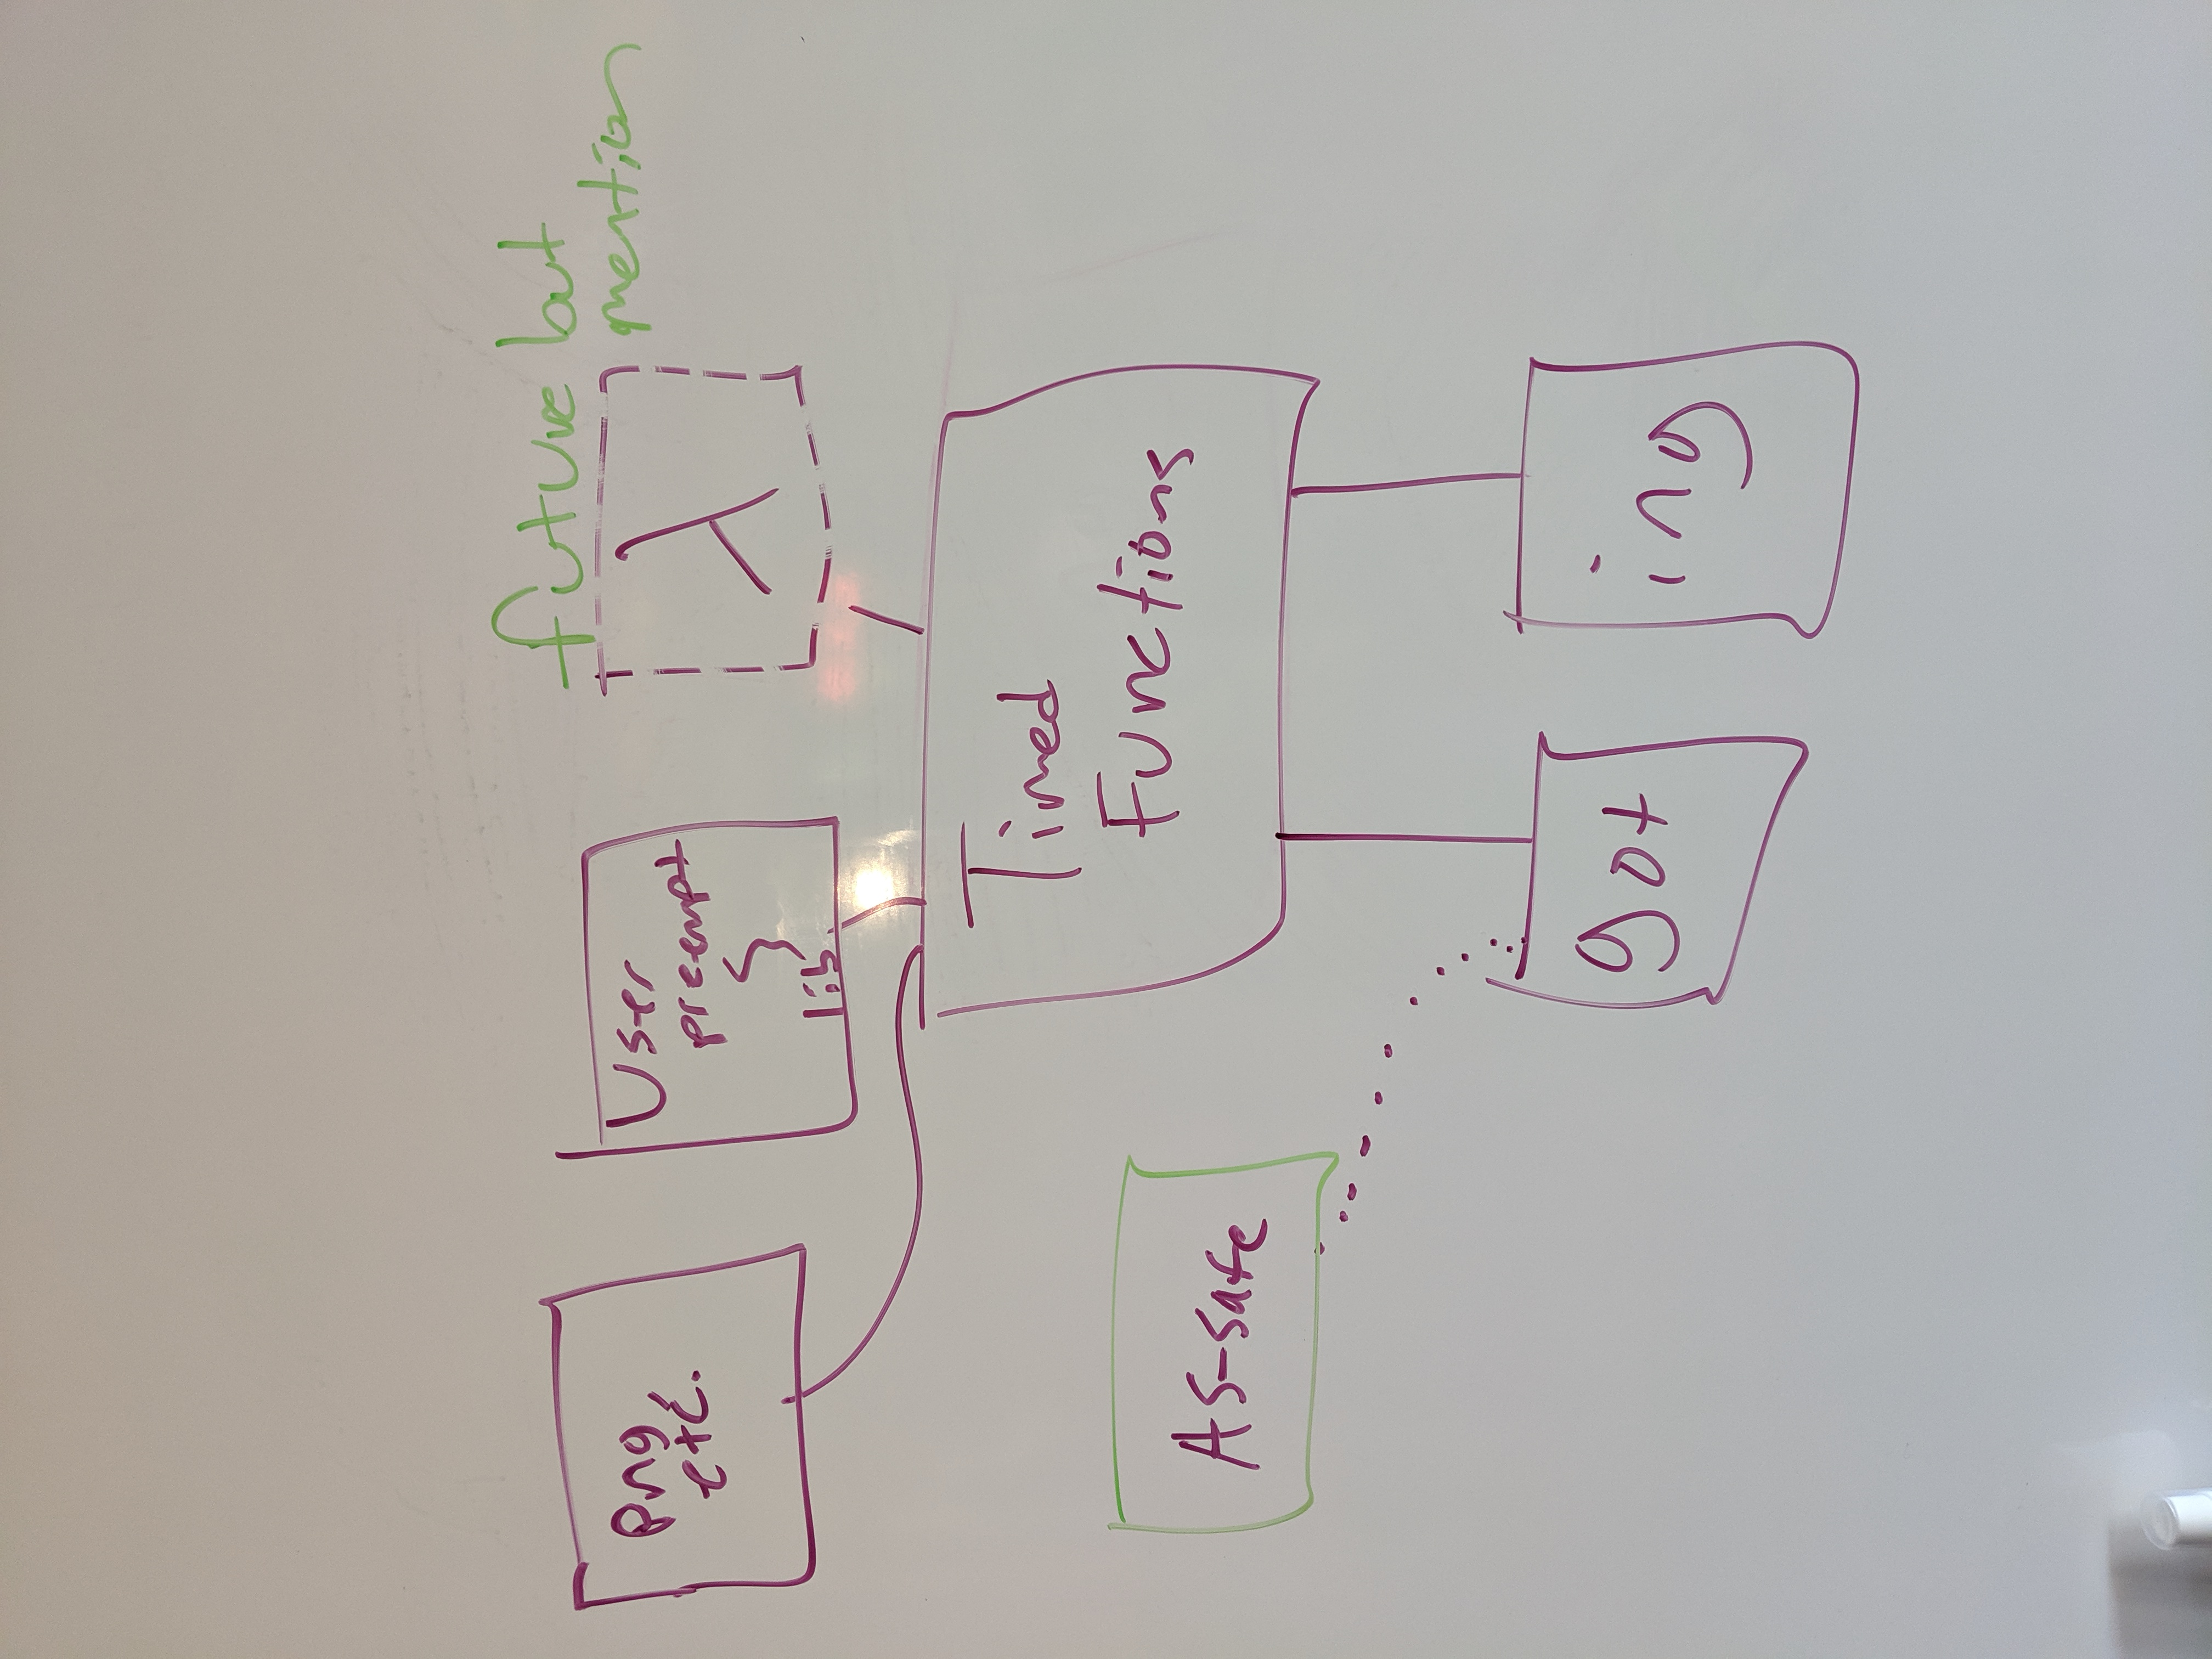
\includegraphics[width=0.75\columnwidth]{figs/architecture}
\end{center}
\caption{The preemptible functions software stack.  \textnormal{Rectangular boxes
represent components implementing the preemptible functions abstraction.  Ovals
represent components built on top of these.  Hexagonal boxes show the
required runtime environment.}}
\label{fig:architecture}
\end{figure}


\subsection{Automatic handling of shared state}

As discussed in Section~\ref{sec:intro}, we wish to design a preemptible
functions library that supports calling third-party libraries without
modification or recompilation. Requiring users to modify such libraries to make
them amenable for \textit{libinger} would greatly limit the usability and convenience
of \textit{libinger}. The central challenge for \textit{libinger} is the \emph{shared
state} problem: Suppose a timed function $\mathcal{F_1}$ calls a stateful
routine in a third-party library $\mathcal{L}$. $\mathcal{F_1}$ times out, and
is preempted by \textit{libinger}. Later the user invokes another timed function
$\mathcal{F_2}$, which also calls a stateful routine in $\mathcal{L}$. The
challenge for us then is to hide state modifications in $\mathcal{L}$ by
$\mathcal{F_1}$ from the execution of $\mathcal{F_2}$.

One non-solution to this problem is to limit functions invocable from
\textit{libinger} to async-signal-safe functions (Section~\ref{sec:related}), because
doing so severely limits the usability of \textit{libinger}. Our solution to this
problem is to automatically and dynamically create copies of $\mathcal{L}$ to
isolate state from different timed functions. Doing so while running on
existing systems software (a requirement discussed next) requires solving many
design and implementation challenges, which we discuss in
Section~\ref{sec:libinger}.


\subsection{Performance on unmodified system stacks}

Unlike prior work on low-latency preemptive scheduling such as
Shinjuku~\cite{Kaffes:nsdi2019}, \textit{libinger} runs on top of the existing
OS. An obvious design to achieve this goal would be to use a thread or process,
the existing concurrency mechanisms provided by the OS, but these mechanisms
are too slow. We choose a middle ground between the very fast but specialized
approaches like Shinjuku, and slow but fully-general OS approaches.


%\subsection{Language independence}
%
%Our interface is inspired by that of Scheme engines~\cite{haynes:iucs1984};
%however, since we seek language independence, there are some fundamental
%differences.  Most notably, our preemptible functions may contain
%state\footnote{In addition to lifting a restriction on timed code, this
%difference led us to make the \texttt{linger} type stateful as well, and allow
%the \texttt{resume()} function to mutate it in place rather than constructing a
%copy.  In another move to improve portability, we chose to make \texttt{linger}
%a structured type instead of a function, thereby avoiding dependence on
%languages supporting closures.  In languages with operator overloading, the
%preemptible function bindings may define a function-call operator that calls
%\texttt{resume()} to achieve Scheme-style surface syntax.}, something not
%handled by Scheme due to the functional nature of the language.  We simplify
%their API by returning the preemptible function's return value in the
%\texttt{linger} union rather than passing it to a success callback.  Our goal
%was to create a core API amenable to language-specific integration integration;
%for instance, in addition to the barebones C interface, our current
%implementation exposes a Rust interface that uses a first-class tagged union
%(sum type) to ensure at compile time that the caller has checked which variant
%a \texttt{linger} contains before using it.
